\documentclass[12pt, git, draft]{rureport}

\usepackage{hyperref}

\begin{document} % this tells the compiler that it is time to make
                 % text to print instead of just getting ready.
\maketitle  % make a title page from the Title, Date, and Author

%\fxnote{skoða titil á skýrslu, sbr. forsíðu}

%\section*{Errata} %%section* avoids putting a number
\listoffixmes 

\section{Inngangur} % sections break up the document into pieces

Markmið verkefnisins er að nota gögn frá Grouplens \cite{movielens} og ná þar í gagnasett sem inniheldur 10 milljón einkunnagjafir og 100 þúsund 'tags' á 10 þúsund kvikmyndum frá 72 þúsund notendum.
\newline
Nemendur áttu svo að útbúa SQL gagnagrunn byggðan á þessum gögnum og skrifa python forrit sem talar við gagnagrunninn.

Forritið á að virka á þann hátt að þegar notandi slær inn heiti á einni eða fleiri kvikmyndum eiga að birtast tillögur að svipuðum myndum.
\section{Framkvæmd}
Byrjað var að nýta minni útgáfu af Grouplens gagnasettinu sem inniheldur "aðeins" 100 þúsund einkunnargjafir á 1700 kvikmyndum. Þetta gagnasett var notað til þess að hægt væri að þróa forrit án þess að keyrslutíminn yrði of langur.

\begin{itemize}
	\item Gögn lesinn inn og forunnin með python
	\begin{itemize}
		\item Ár tekið frá myndum og sett í sér dálk
		\item Gögn úr ratings notuð til að reikna meðaleinkunn hverrar myndar. Meðaleinkunn smellt aftan á upplýsingar um myndir
		\item Genres við hverja mynd aðskilin og sett upp í töflu þar sem key er (genre, mynd), sbr. Mynd \ref{fig:dataschema}
		\item Tög (e. tag) við hverja mynd aðskilin og sett upp í töflu þar sem key er (mynd, tag), sbr. Mynd \ref{fig:dataschema}
	\end{itemize}
	\item Unnin gögn sett upp og hlaðið inn í SQL gagnagrunn á því formi sem sést í Mynd \ref{fig:dataschema}
	\item GUI búið til í Qt4 Designer \cite{qt4}
	\item Queries búnar til fyrir gagnagrunn
	\begin{itemize}
		\item Leit sem finnur genre myndar út frá nafni og ári
		\item Leit sem finnu tög myndar út frá nafni og ári
		\item Leit að svipuðum myndum út frá genres og tags. Meðal-rating "input" mynda notað til að sía niðurstöður
	\end{itemize}
	\item Gluggi sem gerir notanda kleift að slá inn upplýsingar um gagnagrunn búinn til
\end{itemize}

\begin{figure}
	\centering 
	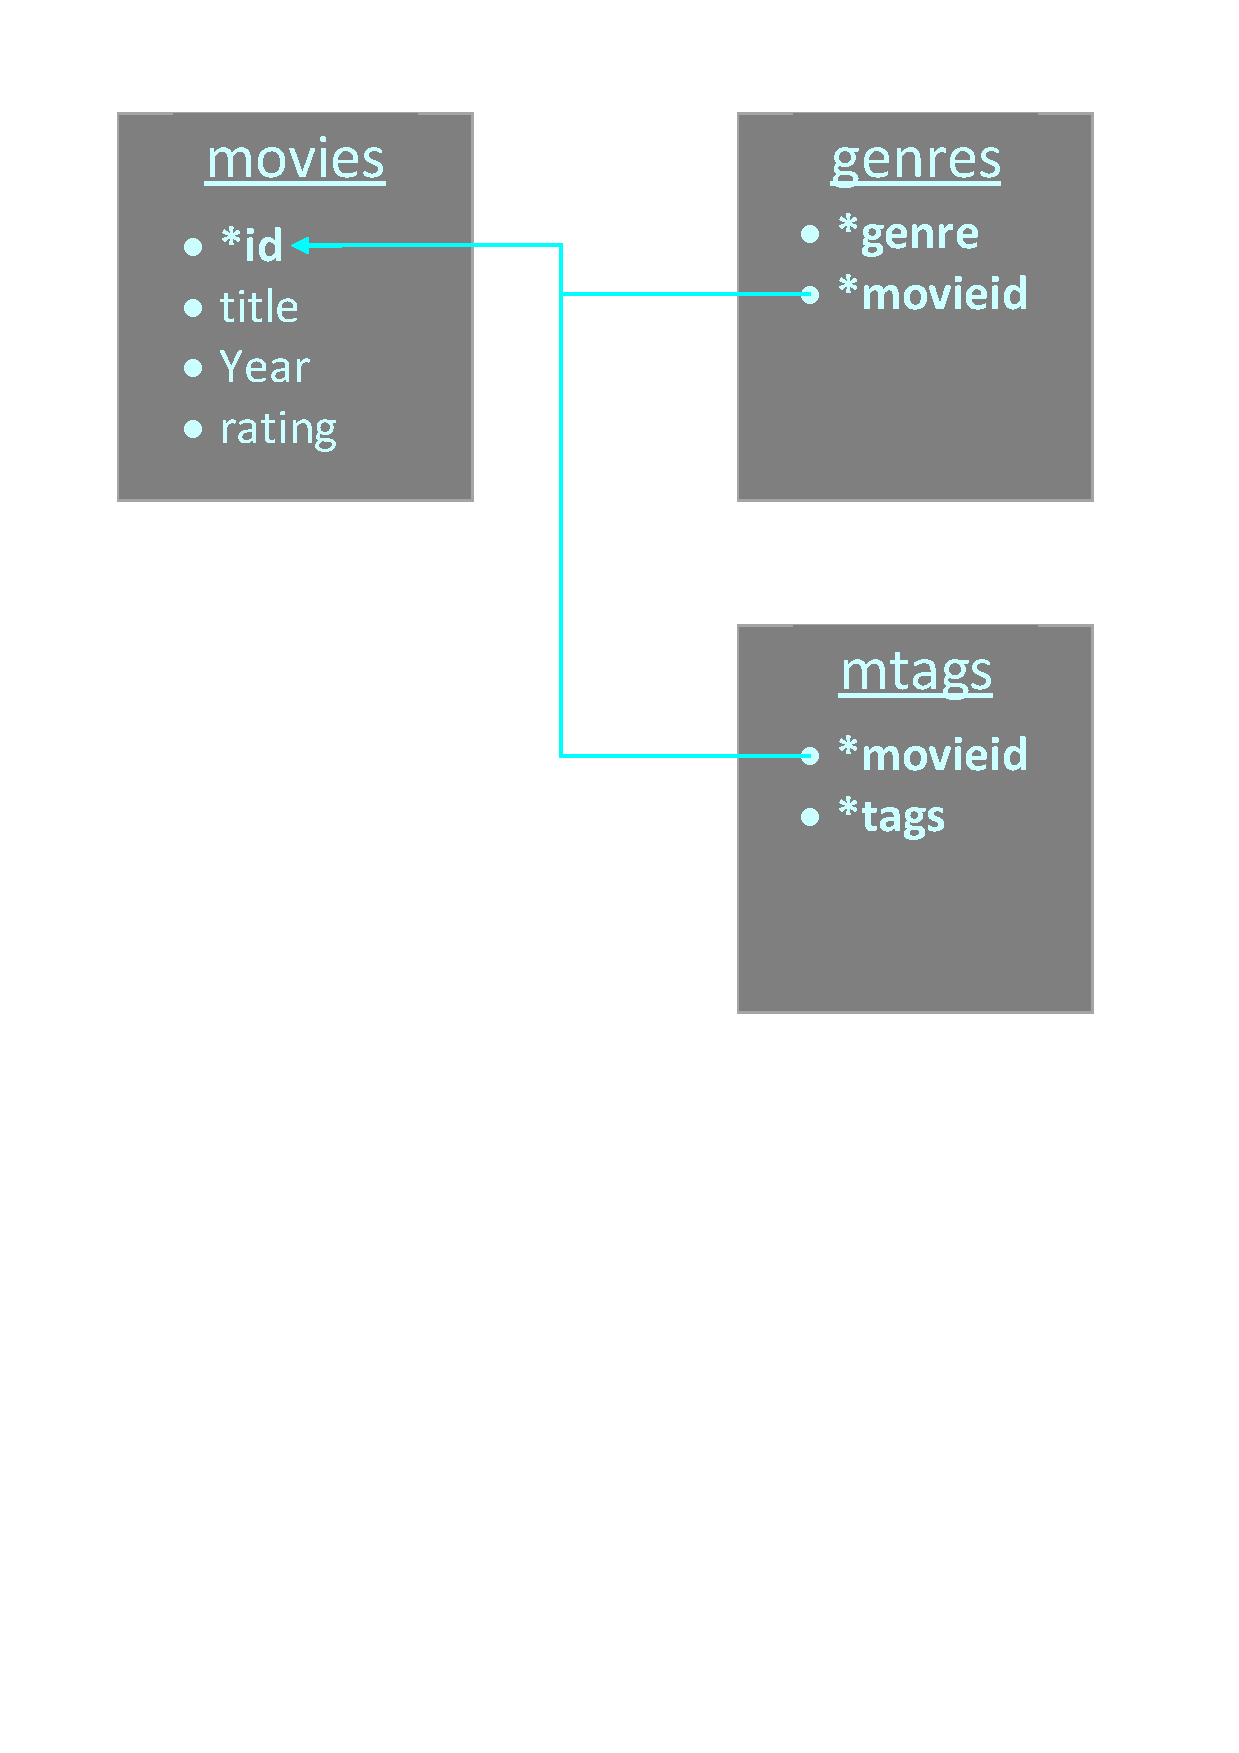
\includegraphics[width=\textwidth, trim = 0pt 11cm 0pt 1cm, clip]{ds.pdf}
	\caption{Database schema \label{fig:dataschema}}
\end{figure} 

\section{Niðurstöður}\label{nidurstodur}
\subsection{Hönnun}
Það var ákveðið að hafa GUI (Graphical user interface) og markmiðið var að hafa það einfalt og sem notendavænast því var búinn til sprettigluggi (sjá mynd \ref{fig:cdbf}), sá gluggi hefur 2 dálka, eina leitarstiku og 5 hnappa. Notast var við Qt4 designer til að hanna GUI, það var valið með þeim áherslum að það var auðvelt í notkun og við yrðum hlutfallslega fljótir að hanna GUI útaf þeim stutta tíma sem nemendur höfðu til að skila verkefninu.
\subsection {Virkni}
Eftir að búið er að keyra gui\_test.py skránna þá opnast gluggi og ýtt er á ctrl+E eða ýtt á Database uppi í hægra horninu og þá myndi opnast annar lítill sprettigluggi þar sem viðeigandi upplýsingar eru skráðar inn til að geta tengst gagnagrunninum í gegnum GUI (sjá mynd \ref{fig:dbf2}), ef það er ekki gert þá poppar upp annar sprettigluggi sem lætur notandan vita að hann eigi eftir að slá inn notendaupplýsingu.
\newline
\newline
Eftir að búið er að slá inn viðeigandi upplýsingar og þær eru réttar þá birtist annar sprettigluggi sem lætur notendan vita að tenging við gagnagrunn hafi tekist, ef upplýsingarnar eru rangar þá kemur sprettiglugginn með upplýsingar að tenging hafi ekki tekist.
\newline
\newline
Þegar notandinn nær að tengjast gagnagrunninum þá getur hann skrifað þá mynd sem hann leitar eftir í leitarstikuna og ýtir svo á search, niðurstöðurnar birtast svo í vinstri dálknum ef notendanum líst svo á einhverja mynd sem koma upp við leitina  getur hann bætt henni við á listan yfir myndir sem hann vill velja, með því að ýta á á 'add' hnappinn og þá dettur myndin í vinstri dálkinn (sjá mynd \ref{fig:dbf6}), þegar ýtt er á 'done' hnappinn þá poppar upp annar spretti gluggi sem kemur með myndir sem þér líkar við (sjá mynd \ref{fig:dbf10}), eftir það er hægt að prófa aðrar myndir með því að ýta á 'yes' hnappinn annar ýtir notandinn á 'no' hnappinn og þá ferðu út úr GUI.

\pagebreak

\begin{figure}
	\centering 
	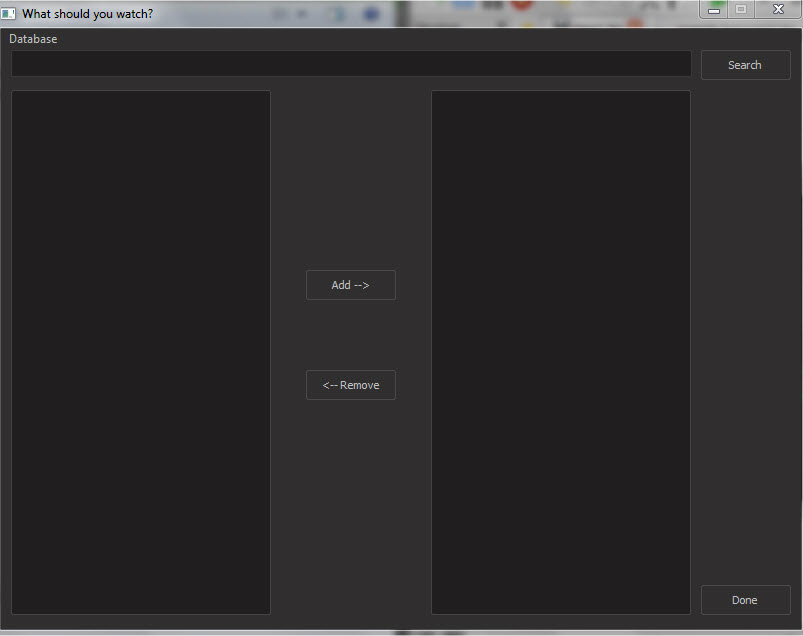
\includegraphics[width=\textwidth]{cdbf.png}
	\caption{Aðalgluggi forritsins \label{fig:cdbf}}
\end{figure}

\begin{figure}
	\centering 
	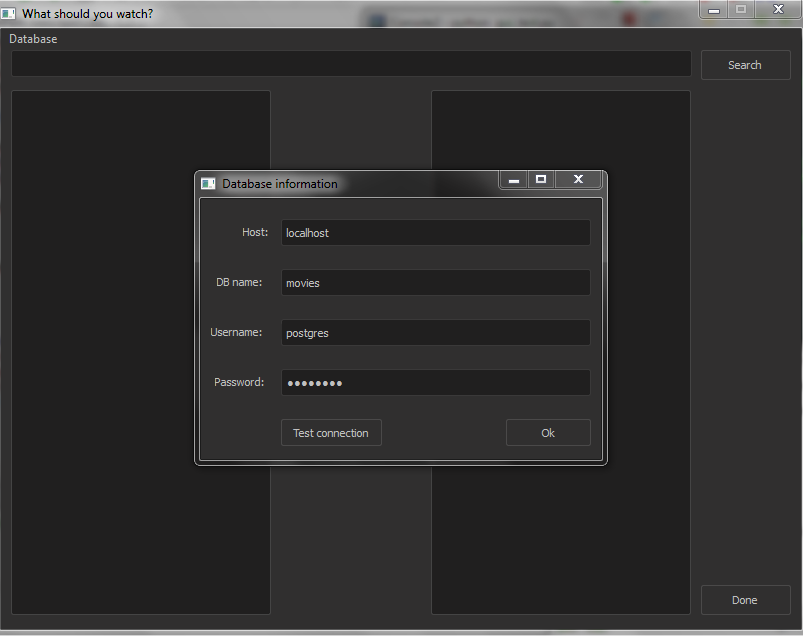
\includegraphics[width=\textwidth]{dbf2.png}
	\caption{Sprettiglugginn með upplýsingum útfylltum \label{fig:dbf2}}
\end{figure}


\begin{figure}
	\centering 
	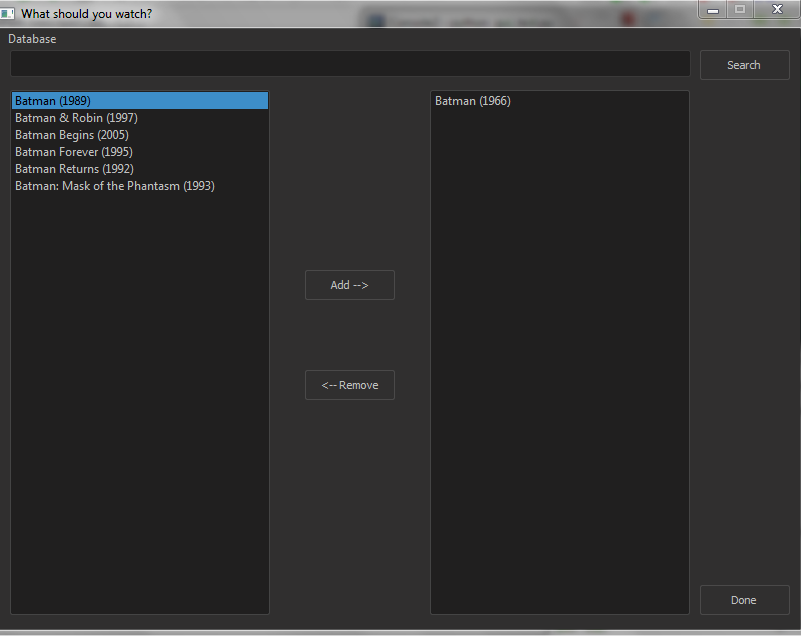
\includegraphics[width=\textwidth]{dbf6.png}
	\caption{Myndaleit skilar niðurstöðum í vinstri dálk\label{fig:dbf6}}
\end{figure}

\begin{figure}
	\centering 
	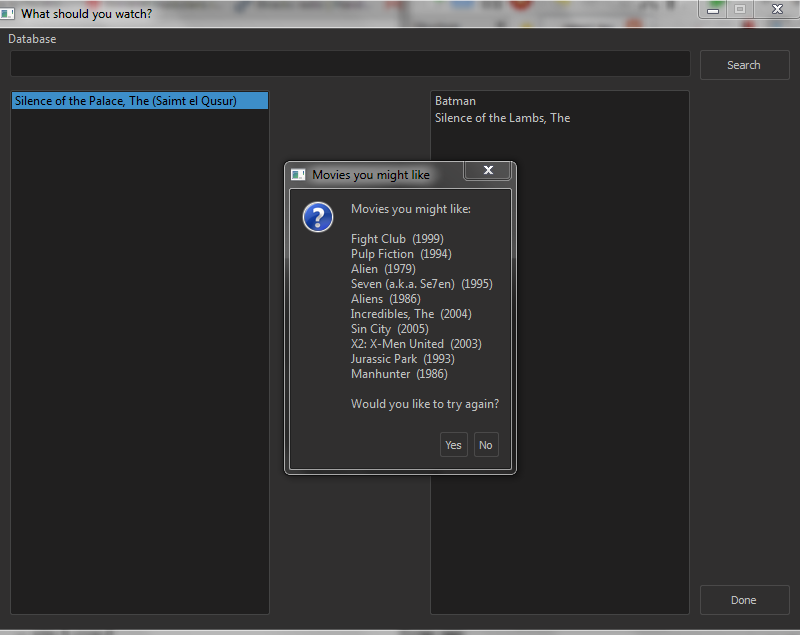
\includegraphics[width=\textwidth]{dbf10.png}
	\caption{Svipaðar myndir og þær sem settar voru í hægri dálkinn birtast í sprettiglugga\label{fig:dbf10}}
\end{figure}

\clearpage
\printbibliography

\end{document} % this tells the compiler that we are done

% These are variables for the editor Emacs
%%% Local Variables: 
%%% TeX-command-BibTeX: biber
%%% mode: latex
%%% TeX-master: t
%%% End:
